O projeto LibrasVision situa-se na interseção entre Visão Computacional, Aprendizado Profundo e acessibilidade linguística, conforme ilustrado na Figura \ref{fig:venn_areas}. Para compreender as escolhas técnicas adotadas, é necessário percorrer o estado da arte nessas áreas, desde os fundamentos do reconhecimento de gestos até os modelos mais avançados de tradução de língua de sinais, com atenção especial ao contexto brasileiro da Língua Brasileira de Sinais (Libras). Revisões sistemáticas recentes confirmam que esse campo está em rápida expansão, com destaque para abordagens baseadas em visão computacional e aprendizado profundo \cite{costa-slr:25, silva-ia:25}. No Brasil, a relevância é amplificada pelo contexto sociolinguístico: a Libras é reconhecida como meio legal de comunicação da comunidade surda brasileira \cite{dockens:18}, e sua inclusão digital depende diretamente do avanço dessas tecnologias assistivas \cite{sousa:25}.

\begin{figure}[htb]
    \centering
    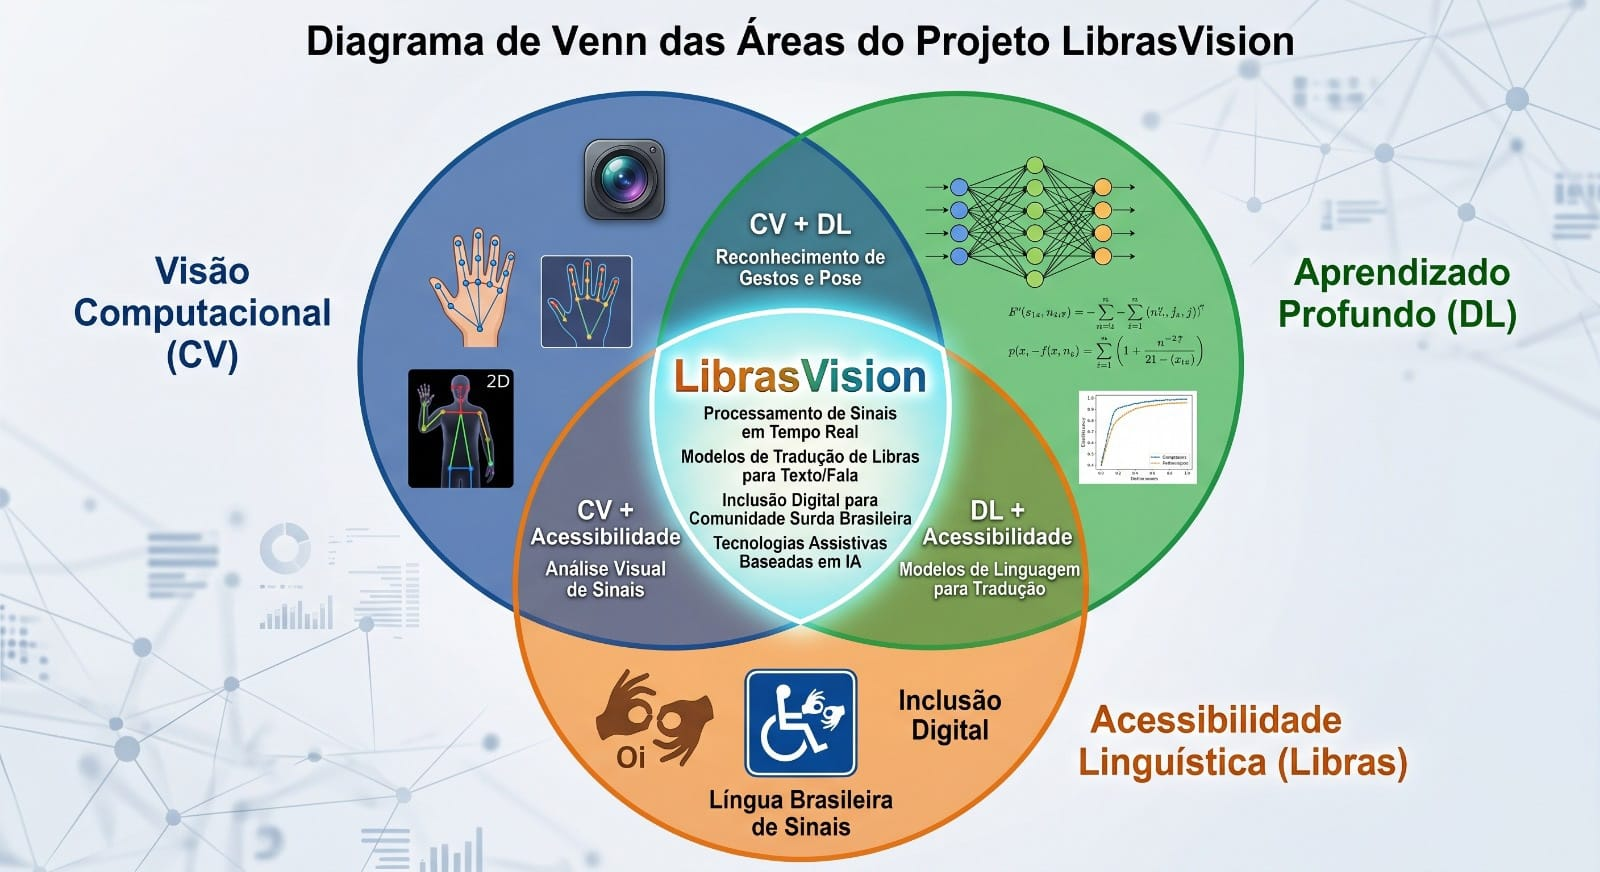
\includegraphics[width=0.75\textwidth]{images/venn_areas.png}
    \caption{Interseção entre Visão Computacional, Aprendizado Profundo e Acessibilidade Linguística no contexto do LibrasVision}
    \label{fig:venn_areas}
\end{figure}

\section{Visão Computacional e Reconhecimento de Gestos}

A Visão Computacional é o campo da Inteligência Artificial que habilita sistemas computacionais a interpretar e compreender o conteúdo de imagens e vídeos digitais. No contexto do reconhecimento de gestos, essa disciplina fornece as ferramentas fundamentais para segmentar regiões de interesse, extrair características relevantes e classificar padrões visuais. Conforme apontado por \citeonline{oudah:20}, em uma revisão abrangente das técnicas da área, os principais desafios do reconhecimento de gestos manuais envolvem segmentação da mão, seleção de algoritmos de classificação e a distinção entre gestos estáticos e dinâmicos, cada um exigindo abordagens metodológicas distintas.

As abordagens tradicionais de reconhecimento de gestos baseiam-se em métodos de comparação temporal, como o \textit{Dynamic Time Warping} (DTW). \citeonline{velmathi:23} demonstraram a eficácia desse método combinado a algoritmos de votação para o reconhecimento de gestos de emergência em tempo real, atingindo alta confiabilidade ao reduzir significativamente os falsos positivos em relação a abordagens de algoritmo único. De forma similar, \citeonline{myagila:25} propuseram um \textit{framework} baseado em diferenças absolutas de estimativa de pose para isolar sinais em vídeos contínuos, alcançando acurácia média de 84\% no reconhecimento de sequências e 95\% no reconhecimento de sinais isolados.

Com o avanço das técnicas de aprendizado de máquina, o rastreamento de pontos-chave do corpo humano (\textit{landmarks}) passou a ser amplamente adotado como representação intermediária, eliminando a necessidade de processar imagens completas. O framework MediaPipe, desenvolvido pelo Google, tornou-se referência nessa abordagem por sua capacidade de extrair centenas de pontos tridimensionais de mãos, rosto e postura corporal em tempo real, com baixo custo computacional. Essa característica é essencial para sistemas embarcados e aplicações que demandam respostas em tempo real \cite{saud:25}.

\section{Aprendizado Profundo para Reconhecimento de Sinais}

As abordagens clássicas de reconhecimento de gestos e língua de sinais dependiam fortemente da engenharia manual de características (\textit{feature engineering}): especialistas definiam descritores de cor, forma, textura ou movimento que o classificador deveria aprender a distinguir. Embora funcionais em condições controladas, esses métodos apresentavam limitações importantes ao lidar com a variabilidade natural dos sinalizadores, variações de iluminação e a complexidade temporal dos sinais dinâmicos, conforme documentado por \citeonline{oudah:20} em revisão abrangente sobre reconhecimento de gestos manuais.

O Aprendizado Profundo (\textit{Deep Learning}) superou essas limitações ao permitir que os próprios modelos aprendam automaticamente, a partir dos dados, quais representações são mais discriminativas para a tarefa. Em vez de features projetadas por humanos, redes profundas constroem hierarquias de representações progressivamente mais abstratas: das bordas e texturas nas camadas iniciais até padrões semânticos complexos nas camadas finais \cite{li:22}. Aplicado ao reconhecimento de língua de sinais, esse paradigma permitiu que sistemas aprendessem diretamente as configurações de mão, trajetórias de movimento e expressões faciais relevantes sem intervenção manual, resultando em ganhos expressivos de acurácia e generalização \cite{grossi:24}. Revisões sistemáticas recentes confirmam que as abordagens baseadas em aprendizado profundo dominam os resultados de estado da arte no reconhecimento de Libras e de outras línguas de sinais \cite{costa-slr:25, silva-ia:25}.

Dentro desse paradigma, duas famílias de arquiteturas se destacam pela complementaridade de suas capacidades, conforme ilustrado na Figura \ref{fig:deeplearning}: as Redes Neurais Convolucionais (CNNs), especializadas na extração de características espaciais a partir de imagens e frames de vídeo \cite{attili:24}; e as Redes de Memória de Curto e Longo Prazo (LSTM), projetadas para modelar dependências temporais em sequências de dados \cite{kamble:25}. As subseções a seguir detalham cada uma dessas arquiteturas e sua aplicação ao reconhecimento de sinais dinâmicos.

\begin{figure}[htb]
    \centering
    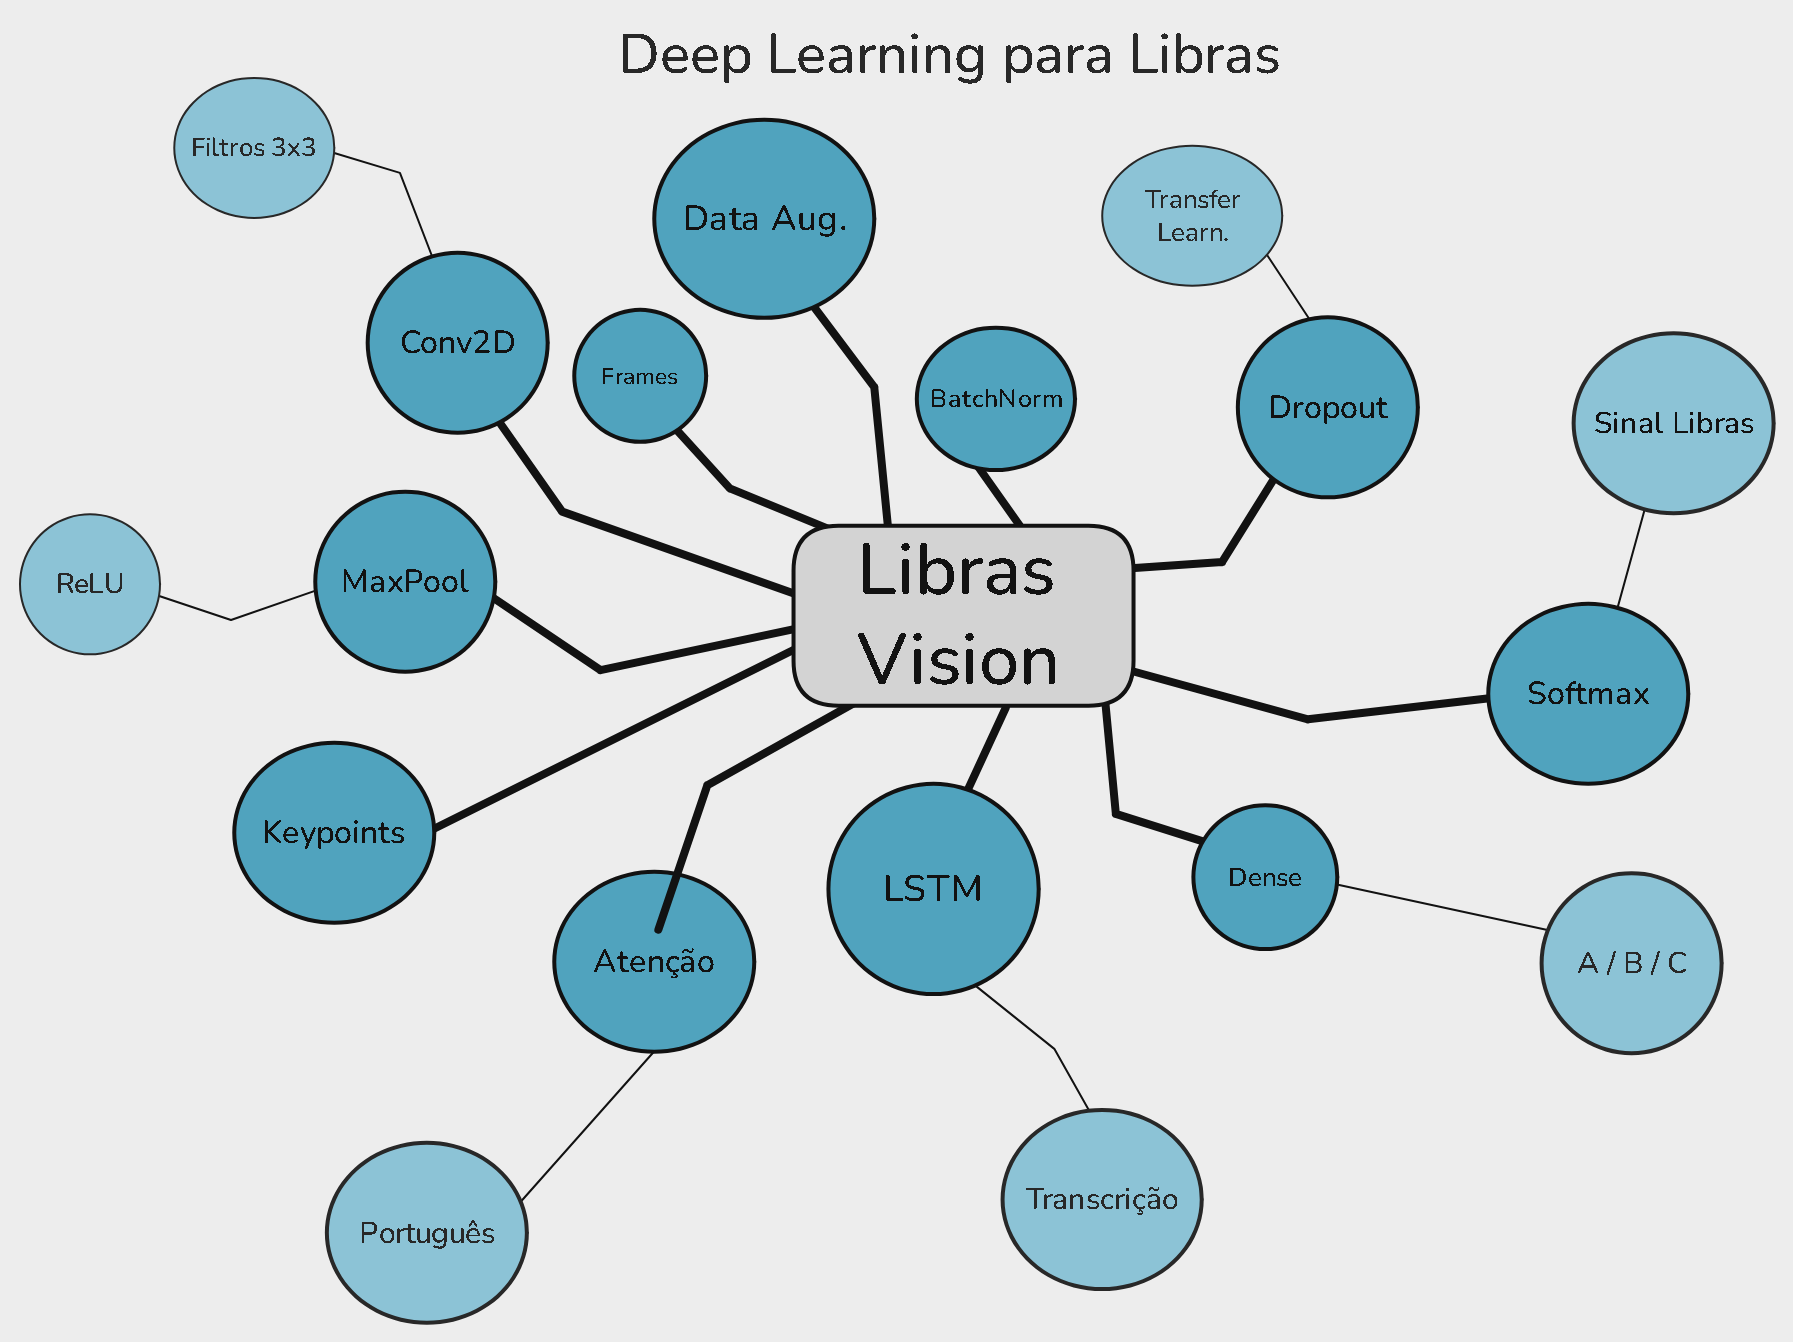
\includegraphics[width=0.8\textwidth]{images/deepL.png}
    \caption{Conceitos de Deep Learning aplicados ao reconhecimento de padrões em dados visuais: da extração automática de características às representações hierárquicas que fundamentam o reconhecimento de língua de sinais}
    \label{fig:deeplearning}
\end{figure}

\subsection{Redes Neurais Convolucionais (CNNs)}

As Redes Neurais Convolucionais (CNNs) são arquiteturas de aprendizado profundo especialmente eficazes na extração de características espaciais em imagens. Sua estrutura típica encadeia camadas convolucionais, que aplicam filtros aprendíveis sobre a entrada para detectar padrões locais como bordas, texturas e formas; camadas de \textit{pooling}, que reduzem a dimensionalidade preservando as características mais relevantes; e camadas totalmente conectadas (\textit{fully connected}), que realizam a classificação final. Conforme \citeonline{li:22}, em survey abrangente sobre CNNs, essa hierarquia de filtros permite que o modelo aprenda representações progressivamente mais abstratas: das bordas simples nas primeiras camadas até configurações complexas de dedos e mãos nas camadas mais profundas (conforme ilustrado na Figura \ref{fig:cnn_architecture}).

No domínio do reconhecimento de gestos e língua de sinais, as CNNs demonstraram resultados expressivos. \citeonline{attili:24} desenvolveram um sistema de tradução da Língua de Sinais Indiana (ISL) em tempo real baseado em CNN, demonstrando que tais sistemas podem alcançar alta acurácia mesmo com hardware convencional, como uma webcam padrão. \citeonline{abdulhussein:20} confirmaram a efetividade de CNNs profundas para classificação de sinais estáticos do alfabeto americano (ASL), e \citeonline{wang:24} expandiram essa aplicação para sistemas inteligentes de aprendizado e promoção de língua de sinais integrados a ambientes educacionais.

A generalização das CNNs pode ser significativamente melhorada por meio de técnicas de aumento de dados (\textit{data augmentation}). \citeonline{islam:19} demonstraram que a aplicação de rotações, zoom e deslocamentos nas imagens de treinamento elevou a acurácia de um modelo CNN de 92,87\% para 97,12\%, evidenciando a importância do pré-processamento de dados para a robustez dos modelos em cenários reais. Complementarmente, \citeonline{sahoo:19} mostraram que a redução de dimensionalidade por Análise de Componentes Principais (PCA) aplicada às \textit{features} extraídas por redes pré-treinadas (como a AlexNet) melhora tanto a acurácia quanto a eficiência computacional de classificadores SVM em tarefas de reconhecimento de gestos. Uma abordagem criativa para Libras foi proposta por \citeonline{alves:24}, que converteu sequências temporais de \textit{landmarks} em imagens 2D e as submeteu a uma CNN simples, superando o estado da arte em acurácia com menor custo de treinamento, estratégia que ilustra a flexibilidade das CNNs mesmo quando aplicadas a representações não-tradicionais.

\begin{figure}[htb]
    \centering
    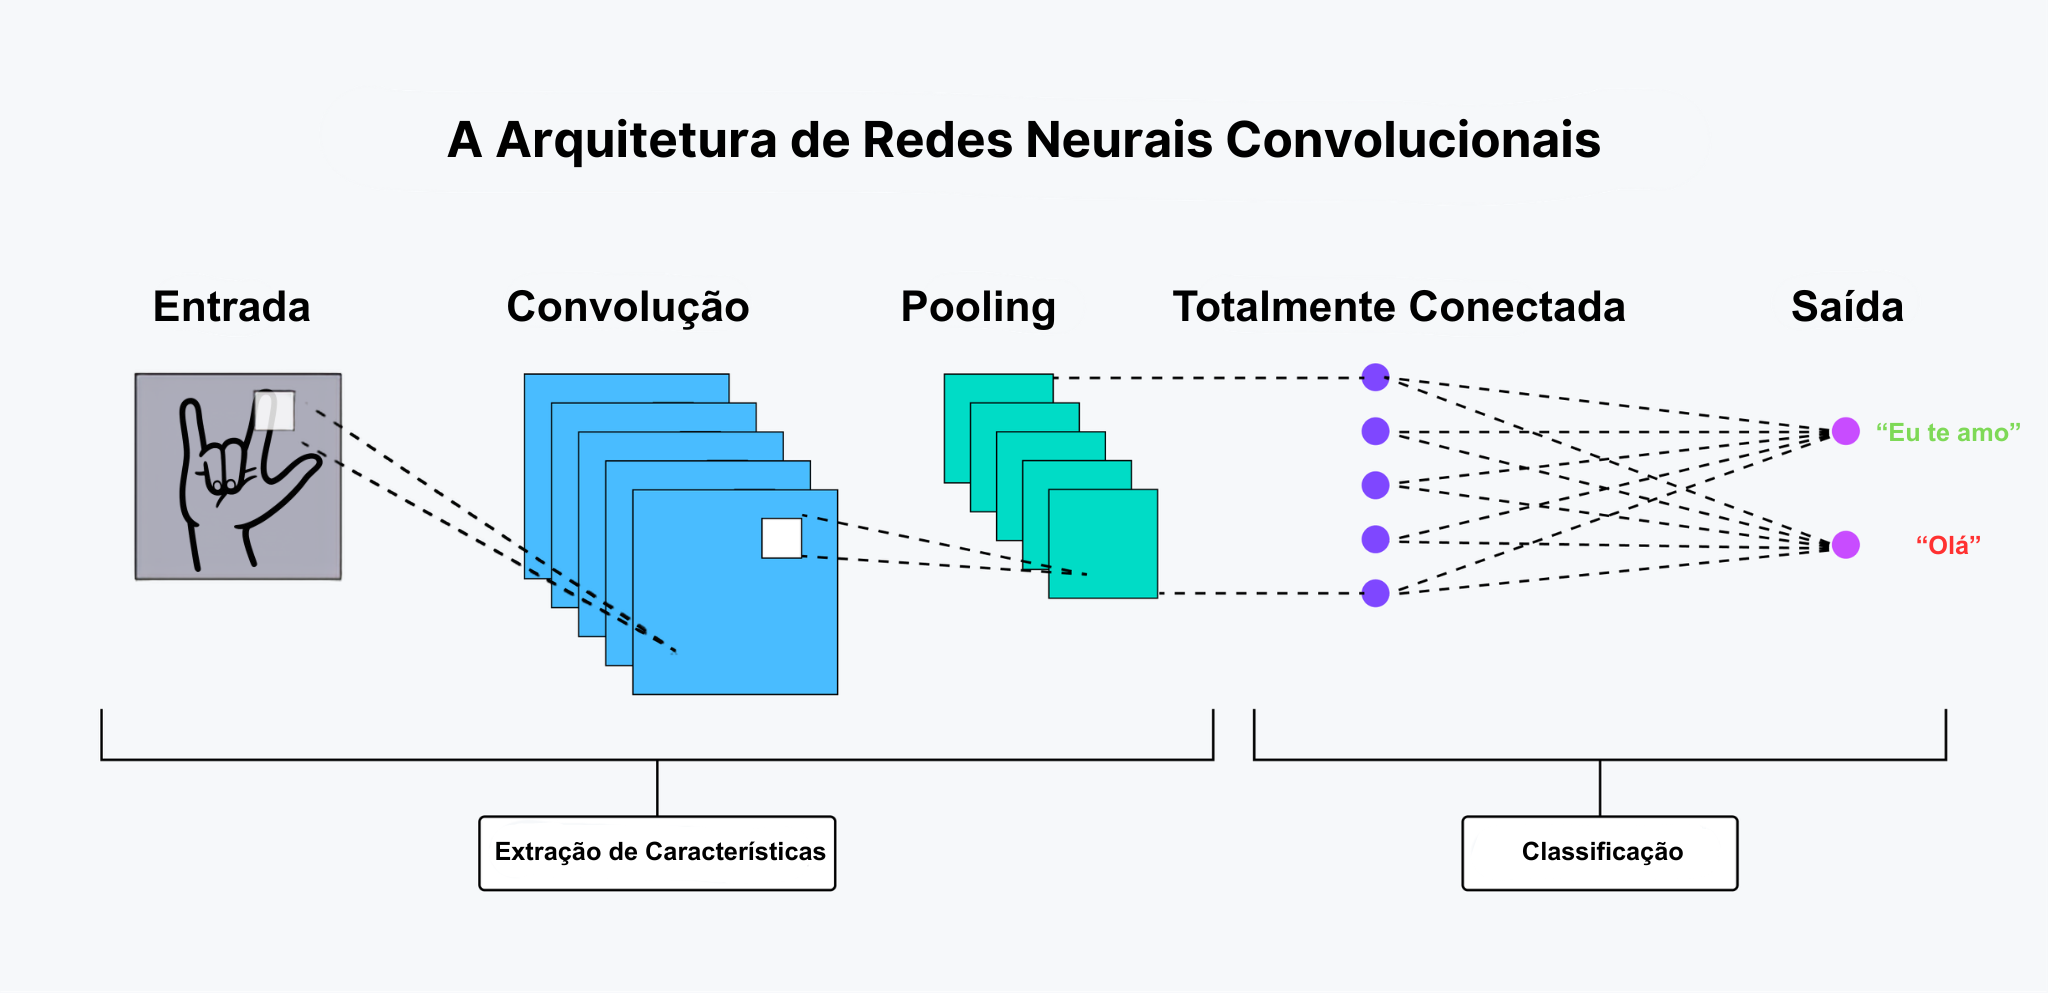
\includegraphics[width=0.85\textwidth]{images/cnn_architecture.png}
    \caption{Arquitetura típica de uma CNN: camadas convolucionais e de \textit{pooling} para extração de características, seguidas de camadas totalmente conectadas para classificação}
    \label{fig:cnn_architecture}
\end{figure}

\subsection{Redes Neurais Recorrentes: LSTM e GRU}

Enquanto as CNNs são excelentes para analisar características espaciais, os sinais dinâmicos de língua de sinais possuem uma dimensão temporal essencial: a mesma configuração de mão pode corresponder a sinais completamente diferentes dependendo do movimento realizado ao longo do tempo. As Redes Neurais Recorrentes (RNNs) foram criadas para modelar exatamente esse tipo de dependência sequencial, mantendo um estado interno que se atualiza a cada passo de tempo. No entanto, as RNNs simples sofrem do problema do \textit{vanishing gradient}: durante o treinamento, o gradiente se torna progressivamente menor à medida que é propagado ao longo de sequências longas, impedindo o aprendizado de dependências temporais distantes.

A arquitetura LSTM (\textit{Long Short-Term Memory}), proposta por Hochreiter e Schmidhuber (1997), resolve esse problema por meio de três portas controláveis: a \textit{forget gate}, que decide quais informações do estado anterior descartar; a \textit{input gate}, que determina quais novas informações armazenar; e a \textit{output gate}, que controla quais partes do estado interno são expostas como saída. Esse mecanismo de memória seletiva permite ao LSTM capturar dependências de longo alcance em sequências de vídeo, tornando-o especialmente adequado ao reconhecimento de língua de sinais \cite{kamble:25, varshini:25}.

A GRU (\textit{Gated Recurrent Unit}) é uma variante simplificada do LSTM que consolida as portas de forget e input em uma única \textit{update gate} e introduz uma \textit{reset gate}, reduzindo o número de parâmetros e o custo computacional sem sacrifício expressivo de desempenho. \citeonline{navendu:24} exploraram diretamente essa complementaridade ao propor uma rede híbrida LSTM-GRU para reconhecimento de ISL ao nível de palavra via MediaPipe, alcançando acurácia de 89,50\% e superando métodos contemporâneos tanto em precisão quanto em velocidade de processamento.

\begin{figure}[htb]
    \centering
    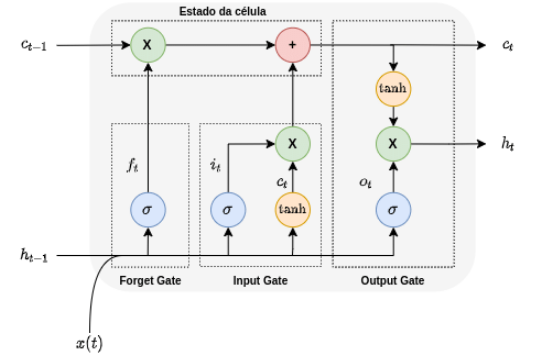
\includegraphics[width=0.80\textwidth]{images/lstm_cell.png}
    \caption{Estrutura interna de uma célula LSTM com suas três portas (forget, input e output) e o \textit{cell state} que persiste ao longo da sequência temporal}
    \label{fig:lstm_cell}
\end{figure}

Na prática do reconhecimento de língua de sinais, o LSTM tem apresentado resultados consistentes, conforme ilustrado na Figura \ref{fig:lstm_unrolled}. \citeonline{kamble:25} introduziram o SLRNet, que combina MediaPipe Holistic com redes LSTM para reconhecimento do alfabeto e palavras funcionais da ASL, atingindo acurácia de validação de 86,7\% sem necessidade de hardware especializado. \citeonline{varshini:25} desenvolveram o MP-GestLSTM com acurácia de 94,38\%, e \citeonline{myagila:25} demonstraram que abordagens baseadas em estimativa de pose aliadas a aprendizado profundo permitem reconhecimento robusto mesmo em vídeos contínuos, atingindo 95\% de acurácia em sinais isolados. A combinação de MediaPipe com LSTM empilhado (\textit{stacked LSTM}) tem se mostrado especialmente poderosa: \citeonline{anithadevi:25} alcançaram 97\% de acurácia e 98,17\% de precisão integrando \textit{landmarks} do MediaPipe com LSTM aprimorado e módulo de paráfrase baseado em Transformer.

\begin{figure}[htb]
    \centering
    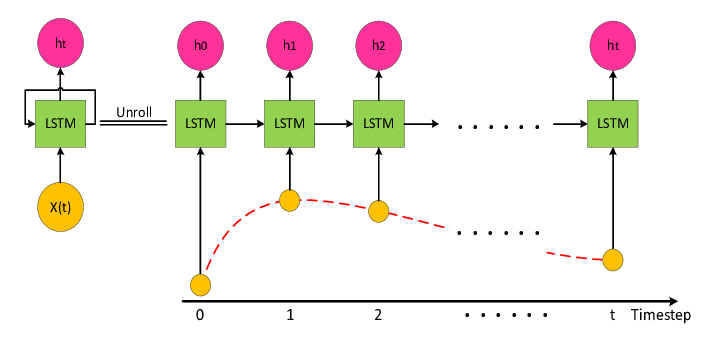
\includegraphics[width=0.85\textwidth]{images/lstm_unrolled.png}
    \caption{LSTM desenrolado no tempo: cada frame da sequência de vídeo alimenta uma célula LSTM, cujo estado oculto é propagado para a célula seguinte até a classificação final do sinal}
    \label{fig:lstm_unrolled}
\end{figure}

\subsection{Arquiteturas Híbridas CNN+RNN}

A combinação de CNNs para extração de características espaciais com RNNs para modelagem temporal representa a abordagem dominante para o reconhecimento de sinais dinâmicos. O funcionamento do pipeline segue uma lógica bem definida: a CNN processa cada frame individualmente, extraindo um vetor de características que encapsula a configuração espacial da mão e do corpo naquele instante; esses vetores são então organizados em uma sequência temporal e fornecidos à RNN (tipicamente um LSTM), que aprende as dependências entre os frames para identificar o padrão de movimento característico de cada sinal. Essa divisão de responsabilidades é eficiente: a CNN abstrai o ``o quê'' (configuração espacial) e a RNN abstrai o ``como'' (evolução temporal), conforme ilustrado na Figura \ref{fig:cnn_lstm_pipeline}.

\citeonline{grossi:24}, em estudo comparativo aplicado à Libras, avaliou modelos CNN+RNN e Transformers para classificação de vídeos de sinais, validando a eficácia do paradigma para classificação temporal. Essa abordagem encontra variações criativas na literatura: \citeonline{alves:24} codificaram sequências temporais de \textit{landmarks} como imagens 2D para processamento por CNN, superando o estado da arte com menor custo de treinamento; \citeonline{costa-i3d:25} adotaram convoluções 3D (\textit{Inflated 3D ConvNet}, I3D), que estendem os filtros convolucionais para a dimensão temporal e operam diretamente sobre vídeos RGB, atingindo 92,5\% de acurácia em Libras sem necessidade de extração de esqueleto. Em abordagem auto-supervisionada, \citeonline{fanucchi:24} exploraram o VideoMAE (\textit{Video Masked Autoencoder}), que aprende representações espaço-temporais ricas a partir de vídeos mascarados, alcançando até 84\% de acurácia em Libras com apenas 50 vídeos de treinamento por palavra, resultado que evidencia o potencial de modelos pré-treinados para cenários com dados escassos. Essa estratégia de encadeamento entre extratores convolucionais e modeladores sequenciais é o fundamento da arquitetura adotada no LibrasVision, conforme detalhado na Seção \ref{sec:arquitetura}.

\begin{figure}[htb]
    \centering
    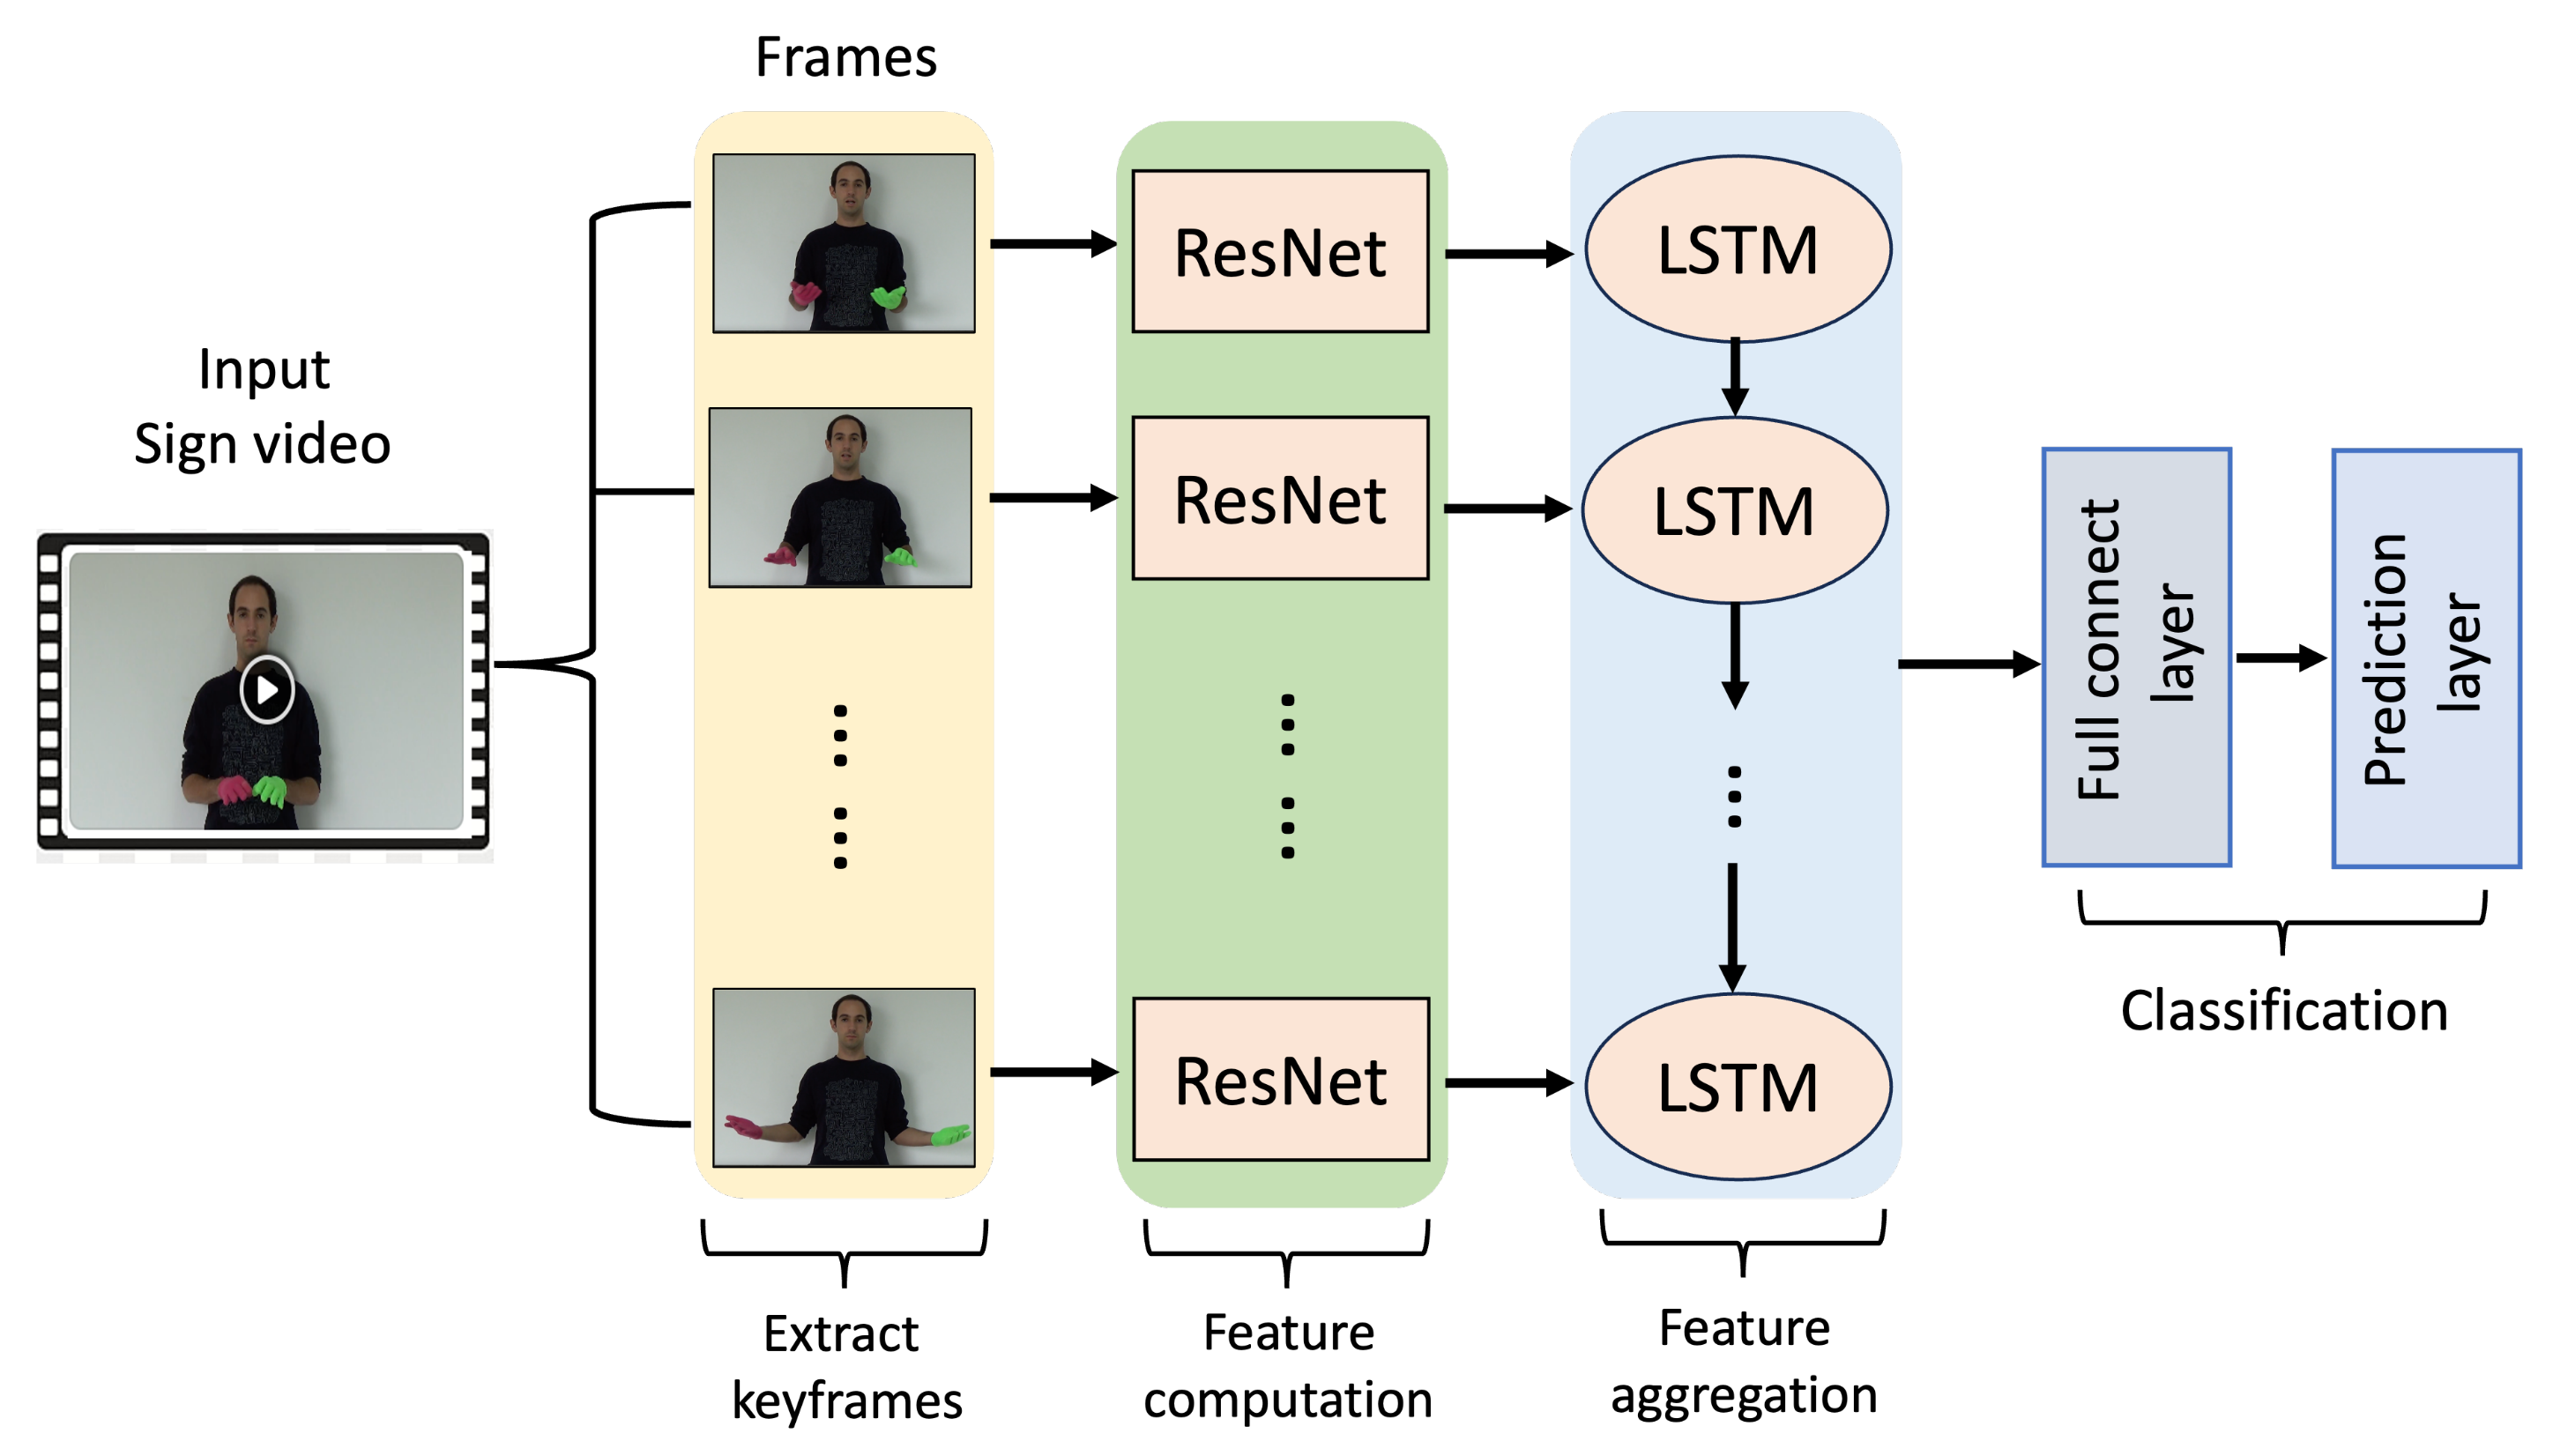
\includegraphics[width=0.90\textwidth]{images/cnn_lstm_pipeline.png}
    \caption{Pipeline CNN+LSTM para reconhecimento de sinais dinâmicos: frames de vídeo são processados pela CNN para extração de características, que alimentam o LSTM para modelagem temporal e classificação final}
    \label{fig:cnn_lstm_pipeline}
\end{figure}

\section{Modelos Avançados de Tradução de Sinais}

A fronteira mais avançada do reconhecimento e tradução de língua de sinais incorpora arquiteturas Transformer, modelos de visão mascarada e abordagens multilingues, que ampliam significativamente as capacidades dos sistemas baseados em LSTM.

\subsection{Transformers e Mecanismos de Atenção}

Os modelos Transformer, baseados em mecanismos de auto-atenção (\textit{self-attention}), demonstraram superioridade na captura de dependências temporais de longo alcance em comparação com LSTMs tradicionais. \citeonline{maia:25} apresentaram uma arquitetura Transformer para tradução de língua de sinais para texto utilizando embeddings de pontos-chave extraídos via MediaPipe Holistic, mostrando que o mecanismo de auto-atenção é superior ao LSTM na captura de dependências temporais de longo alcance. \citeonline{jain:24} integraram CNNs e Transformers para criar um sistema bidirecional de tradução ASL-Inglês com interface de avatar animado, inovando ao suportar chamadas de vídeo com tradução em tempo real. O sistema desenvolvido por \citeonline{mdpi:25} também adota uma arquitetura híbrida CNN-Transformer para tradução bidirecional, atingindo WER (\textit{Word Error Rate}) de 25,17\% no benchmark Phoenix e ROUGE-L de 96,00 na geração de gloss.

\subsection{Eficiência Computacional e Abordagens Multi-stream}

Uma limitação importante dos modelos de tradução de sinais em larga escala é o alto custo computacional de treinamento e inferência. \citeonline{gueuwou:25} propuseram o SignMusketeers, um método eficiente em dados e processamento que aprende representações de configurações de mão e expressões faciais de forma autossupervisionada a partir de frames individuais, sem rastreamento de pose pesado, alcançando performance competitiva utilizando menos de 3\% do poder computacional de modelos anteriores do estado da arte.

\subsection{Tradução Multilingue}

A escassez de dados rotulados é um dos principais obstáculos ao desenvolvimento de sistemas de reconhecimento e tradução para línguas de sinais menos representadas, como a Libras. Enquanto a ASL e a ISL contam com datasets de maior escala e comunidades de pesquisa estabelecidas, a Libras carece de corpora comparáveis, lacuna documentada nas revisões sistemáticas de \citeonline{costa-slr:25} e \citeonline{silva-ia:25}. Nesse contexto, estratégias multilingues e de transferência de aprendizado ganham relevância como caminhos para aproveitar representações aprendidas em línguas de sinais com mais dados e adaptá-las a línguas com recursos escassos.

A abordagem de tradução bidirecional desenvolvida por \citeonline{jain:24}, que converte tanto de língua de sinais para texto quanto de texto para sinais via avatar animado, demonstra que arquiteturas multimodais podem ser projetadas para suportar múltiplas línguas de sinais com adaptações modulares. De forma similar, \citeonline{mdpi:25} propuseram um sistema híbrido CNN-Transformer para tradução bidirecional entre ASL e inglês cuja estrutura modular favorece a extensão para outros idiomas.

No campo da tradução multilingue propriamente dita, \citeonline{maia:25} demonstraram que arquiteturas Transformer com embeddings de \textit{landmarks} extraídos via MediaPipe são capazes de generalizar representações semânticas de sinais entre diferentes contextos linguísticos. O avanço mais direto sobre o desafio de baixos recursos foi proposto por \citeonline{hamidullah:25} com o SONAR-SLT: o sistema emprega embeddings multimodais agnósticos à língua, pré-treinados em texto e fala de dezenas de idiomas, para supervisionar a tradução de língua de sinais sem depender de grandes corpora sinalizados, demonstrando melhorias consistentes especialmente em cenários de poucos dados. Essa linha de pesquisa é particularmente relevante para a Libras, cujo avanço tecnológico depende de estratégias que compensem a assimetria de recursos em relação às línguas de sinais mais estudadas.

\begin{figure}[htb]
    \centering
    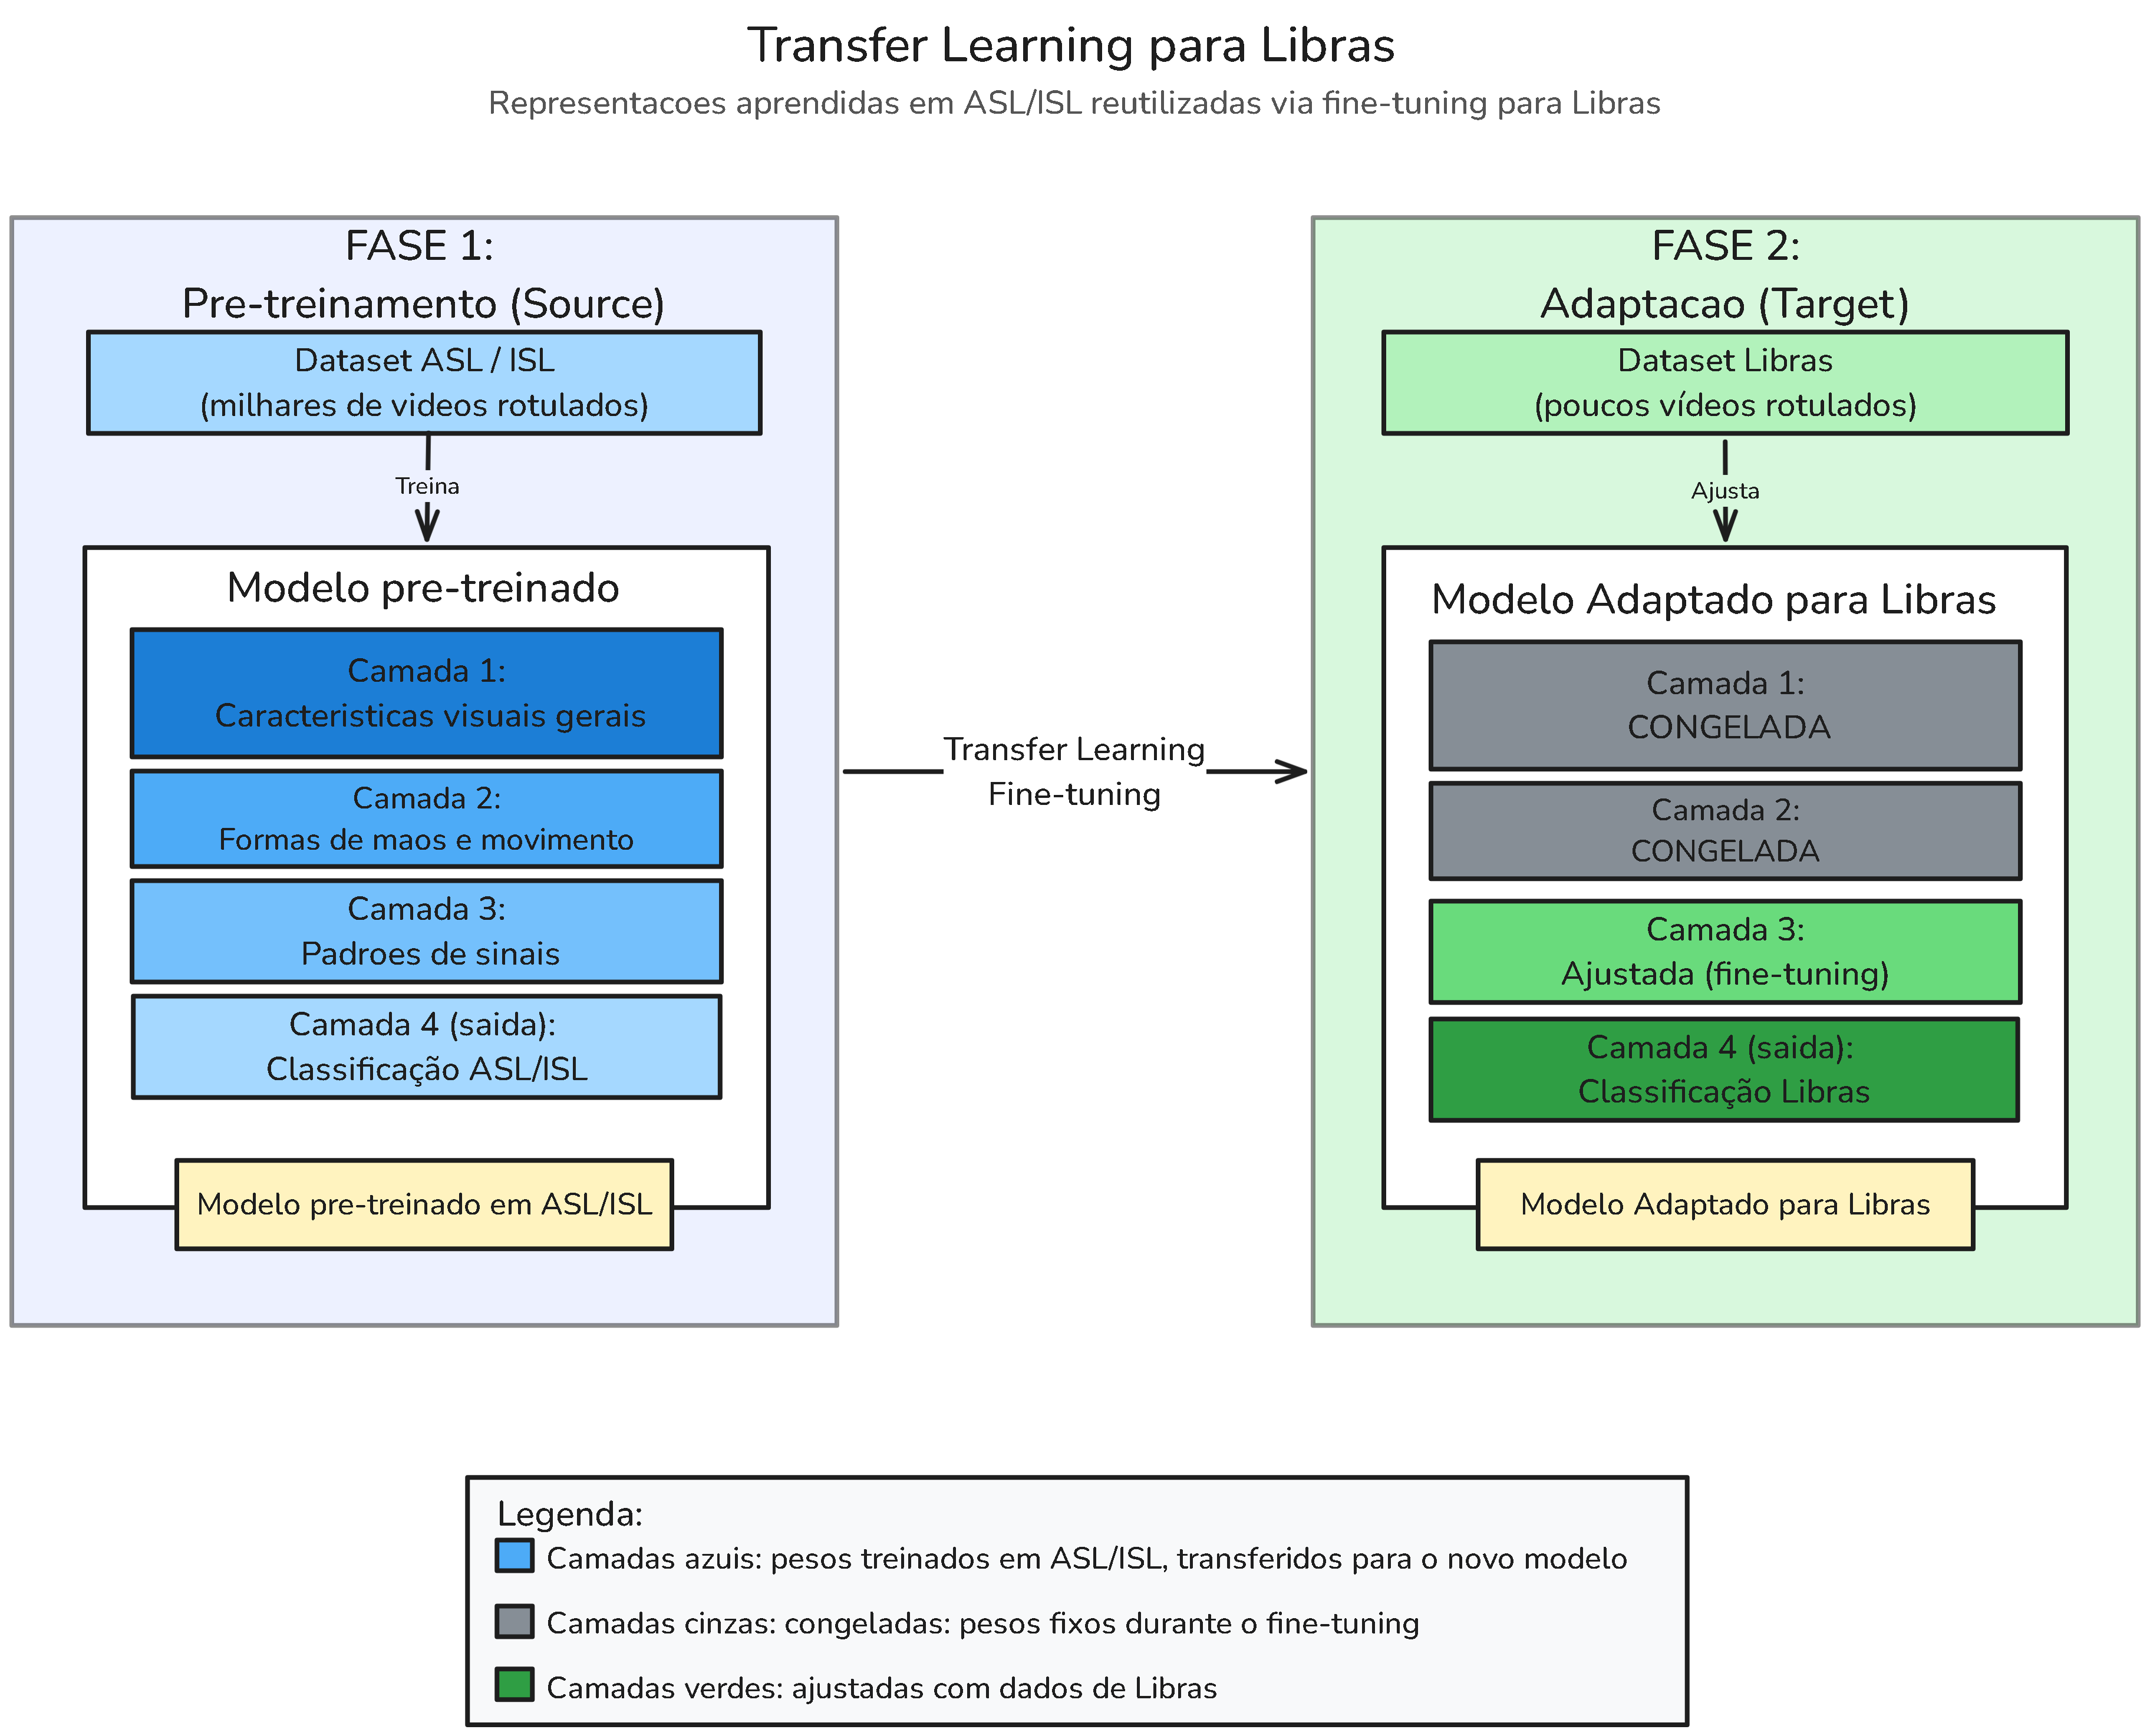
\includegraphics[width=0.80\textwidth]{images/transfer_learning_sl.png}
    \caption{Transferência de aprendizado entre línguas de sinais: representações aprendidas em ASL/ISL são reutilizadas e refinadas (\textit{fine-tuning}) para Libras, reduzindo a necessidade de dados rotulados}
    \label{fig:transfer_learning_sl}
\end{figure}

\section{Reconhecimento de Língua de Sinais: Contexto Internacional}

O campo do reconhecimento automático de língua de sinais tem se desenvolvido principalmente com foco em idiomas como ASL (Língua de Sinais Americana) e ISL (Língua de Sinais Indiana), que contam com datasets maiores e comunidades de pesquisa mais estabelecidas. Essa literatura internacional fornece bases metodológicas diretamente aplicáveis ao reconhecimento da Libras.

Os sistemas de tradução em tempo real evoluíram de abordagens centradas em gestos estáticos para o reconhecimento de sinais dinâmicos completos. \citeonline{attili:24} demonstraram que sistemas baseados em visão computacional e aprendizado de máquina podem traduzir sinais da ISL para texto e fala em tempo real com baixa latência, sendo independentes de hardware especializado, requisito essencial para acessibilidade ampla. \citeonline{scitepress:25} ampliaram essa perspectiva ao integrar reconhecimento de gestos com módulos de Processamento de Linguagem Natural (PLN), criando um sistema multimodal capaz de fornecer saída simultânea em texto e fala, projetado para ambientes de saúde, educação e serviços públicos.

Para o reconhecimento de sinais contínuos, desafio distinto do reconhecimento de sinais isolados, \citeonline{myagila:25} propuseram uma abordagem baseada em diferenças de estimativa de pose para segmentar automaticamente os sinais em vídeos contínuos, superando a abordagem de janela deslizante ao reduzir classificações desnecessárias. A tradução bidirecional, que permite tanto a leitura quanto a produção de sinais, representa outra fronteira importante: \citeonline{jain:24} e \citeonline{mdpi:25} desenvolveram sistemas capazes de traduzir de língua de sinais para texto e vice-versa, com suporte a avatares animados e integração com chamadas de vídeo.

\section{Libras e Tecnologias Assistivas no Brasil}

A Língua Brasileira de Sinais (Libras) apresenta características linguísticas próprias que a distinguem de outras línguas de sinais, incluindo estrutura gramatical visual-gestual com uso intenso de expressões não-manuais (expressões faciais e movimentos de cabeça) como marcadores gramaticais, conforme ilustrado na Figura \ref{fig:libras}. Segundo estimativas do IBGE, mais de 10 milhões de brasileiros possuem algum grau de deficiência auditiva, evidenciando a relevância social de sistemas que facilitem a comunicação desse público \cite{sousa:25}.

\begin{figure}[htb]
    \centering
    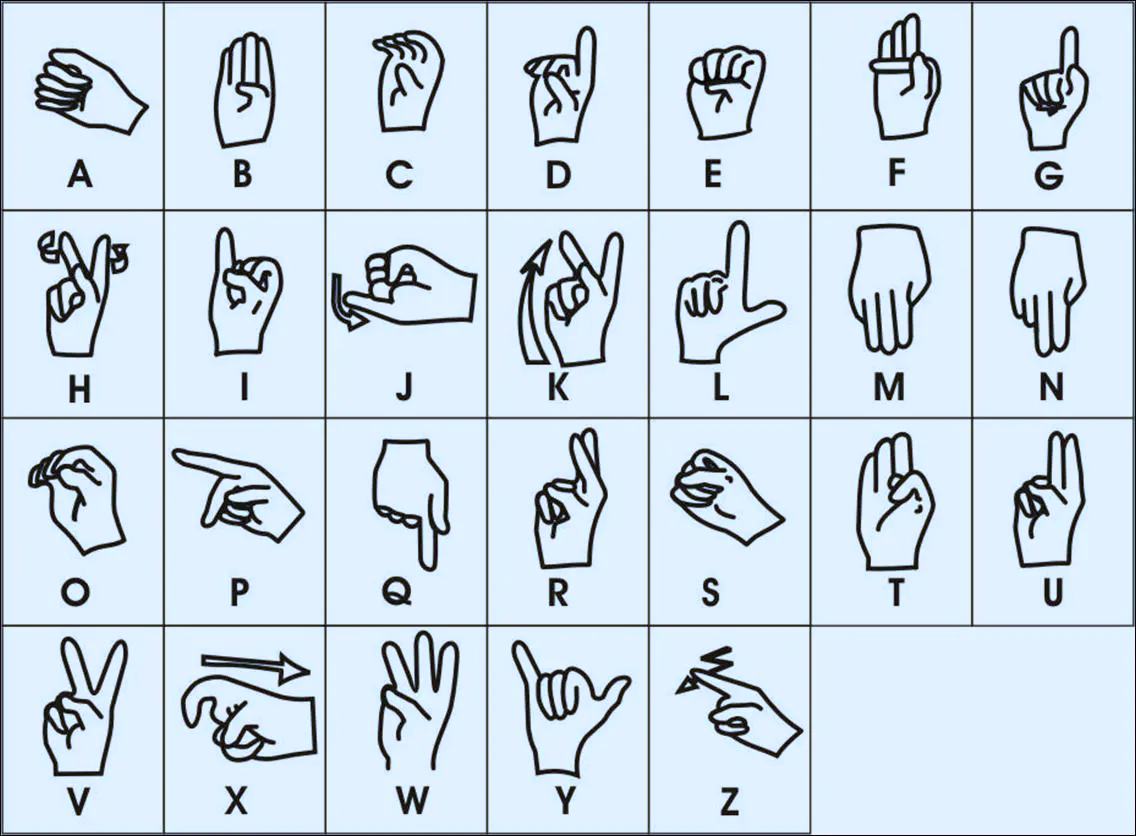
\includegraphics[width=0.8\textwidth]{images/libras.png}
    \caption{Exemplos de sinais dinâmicos na Língua Brasileira de Sinais}
    \label{fig:libras}
\end{figure}

\subsection{Datasets de Libras}

A disponibilidade de datasets de qualidade é um pré-requisito fundamental para o desenvolvimento de sistemas robustos de reconhecimento de Libras. \citeonline{lobo-neto:24} apresentaram o LSWH100, um dataset com 144.000 imagens sintéticas fotorrealistas de mãos humanas cobrindo 100 classes de configurações de mão da Libras, utilizando a convenção SignWriting. As imagens foram geradas via software Blender com variações de iluminação, fundo e tom de pele, e incluem anotações para classificação, detecção, segmentação e pontos-chave 3D. Apesar do avanço representado, os próprios autores ressaltam a necessidade de validação com dados reais de sinalizadores humanos.

Para o reconhecimento de sinais contínuos em vídeo, \citeonline{costa-i3d:25} propuseram um pipeline leve baseado no modelo I3D (\textit{Inflated 3D ConvNet}) aplicado ao dataset MINDS-Libras, operando diretamente sobre vídeos RGB sem extração de esqueleto. Adotando um protocolo rigoroso de avaliação independente de sinalizador, em que os participantes do teste não são vistos durante o treinamento, o sistema atingiu acurácia de 92,5\% em tempo real. \citeonline{alves:24} desenvolveram uma abordagem alternativa em que \textit{landmarks} de corpo, mãos e face são extraídos ao longo do tempo e codificados como imagens 2D para processamento por uma CNN simples, superando o estado da arte em acurácia com menor custo de treinamento. \citeonline{fanucchi:24} exploraram o potencial do VideoMAE (\textit{Video Masked Autoencoder}) para Libras, aplicando \textit{fine-tuning} do modelo no dataset MINDS-Libras para integração com dispositivos de realidade aumentada, atingindo até 84\% de acurácia com apenas 50 vídeos de treinamento por palavra.

\subsection{Aplicações Educacionais e Assistivas}

No contexto educacional, diversas iniciativas têm explorado a IA para facilitar o aprendizado e a comunicação em Libras. \citeonline{lia:25} desenvolveram o aplicativo LIA (\textit{Libras com Inteligência Artificial}), que utiliza reconhecimento de gestos em tempo real para validar o aprendizado de sinais pelo usuário, incorporando elementos de gamificação para engajamento contínuo e processamento local no dispositivo móvel sem necessidade de conexão com a nuvem. \citeonline{silva-conexao:24} criaram a ferramenta Conexão Linguística, um software web baseado em JavaScript para leitura e interpretação de sinais gramaticais da Libras, focando na acessibilidade linguística em ambientes educacionais e profissionais.

Abordagens com hardware de baixo custo também têm sido investigadas para ampliar a acessibilidade. \citeonline{silva-embarcado:24} demonstraram a viabilidade de sistemas integrados entre visão computacional e microcontroladores, com CNNs otimizadas para rodar localmente em dispositivos portáteis, reconhecendo as letras do alfabeto manual com precisão satisfatória para fins de comunicação básica. \citeonline{perdigoto:24} realizaram um estudo prático utilizando OpenCV e OpenPose para detecção de keypoints da mão, atingindo 65,51\% de acurácia com imagens padronizadas, mas com queda drástica para 6,97\% com imagens de usuários leigos, evidenciando a importância de bases de dados diversificadas.

\subsection{Revisões Sistemáticas e Estado da Arte em Libras}

As revisões sistemáticas da literatura sobre Libras e IA fornecem um panorama abrangente do campo. \citeonline{costa-slr:25}, em uma Revisão Sistemática da Literatura (RSL) seguindo o protocolo PRISMA, analisaram 23 estudos selecionados sobre aplicações de Visão Computacional e PLN para Libras, identificando avanços significativos em arquiteturas de aprendizado profundo, mas persistência de desafios em sinais contínuos e características não-manuais. \citeonline{silva-ia:25} revisaram 34 trabalhos publicados entre 2019 e 2025, sistematizando as contribuições em três eixos: aplicativos de tradução automática, tecnologias assistivas e ensino, e reconhecimento por visão computacional. Os autores identificaram um campo em rápida expansão, com destaque para Deep Learning e Realidade Aumentada, mas com desafios persistentes em naturalidade linguística e implicações éticas. \citeonline{sousa:25} reforçaram essa perspectiva ao destacar que, apesar do potencial da IA para superar barreiras de comunicação, a baixa expressividade de avatares digitais e a falta de datasets que cubram a complexidade semântica completa da Libras permanecem como obstáculos centrais.

\section{Estado da Arte e Lacunas Identificadas}

A análise da literatura permite identificar um campo em acelerada evolução, mas com lacunas importantes que motivam o desenvolvimento do LibrasVision. No que diz respeito ao desempenho técnico, modelos baseados em MediaPipe+LSTM têm atingido resultados expressivos: acurácia de 97\% \cite{anithadevi:25}, 94,38\% \cite{varshini:25} e 92,5\% \cite{costa-i3d:25} em diferentes contextos e línguas de sinais. Contudo, esses resultados são frequentemente obtidos em condições controladas, com sinalizadores específicos vistos durante o treinamento e vocabulários limitados.

As principais lacunas identificadas nas revisões sistemáticas \cite{costa-slr:25,silva-ia:25,silva-libras:25} incluem: (1) escassez de datasets de larga escala e multimodais para Libras, que cubram a diversidade de sinalizadores, regiões geográficas e variações de iluminação; (2) dificuldade em integrar características não-manuais (expressões faciais e movimentos de cabeça) como marcadores gramaticais nos modelos de reconhecimento; (3) limitações no reconhecimento de sinais contínuos em conversação natural, que é substancialmente mais complexo que o reconhecimento de sinais isolados; e (4) necessidade de maior atenção às implicações éticas do uso de dados sensíveis de pessoas surdas. Essas lacunas orientam as escolhas metodológicas e as delimitações do escopo do LibrasVision, descritas nas seções seguintes.

\section{Arquitetura do Sistema}
\label{sec:arquitetura}

O sistema proposto será estruturado em um pipeline dividido em etapas bem definidas. A arquitetura a ser adotada seguirá o padrão estabelecido na literatura de maior desempenho: extração de landmarks via MediaPipe seguida de modelagem temporal via LSTM \cite{kamble:25,varshini:25,anithadevi:25,navendu:24,maia:25}.

\subsection{Aquisição de Dados}

A primeira etapa consistirá na captura de vídeo em tempo real por meio de uma webcam convencional, operando a aproximadamente 30 quadros por segundo (FPS). A independência de hardware especializado é uma característica deliberada do projeto: conforme demonstrado por \citeonline{attili:24} e \citeonline{kamble:25}, sistemas baseados em webcam padrão são viáveis para tradução de língua de sinais em tempo real, tornando a solução acessível a diferentes contextos socioeconômicos.

\subsection{Extração de Características}

Nesta fase, será utilizado o framework MediaPipe Holistic, responsável por identificar e rastrear pontos-chave do corpo humano (\textit{landmarks}), incluindo mãos, rosto e tronco. Ao todo, serão extraídos 543 pontos tridimensionais (x, y, z) por frame: 33 pontos de pose corporal, 21 pontos por mão (42 no total) e 468 pontos faciais. Essa representação reduzirá significativamente a necessidade de processar imagens completas, tornando o sistema mais eficiente e preservando a privacidade dos usuários ao não armazenar dados de imagem \cite{varshini:25,anithadevi:25,maia:25}.

\subsection{Modelagem Temporal}

Os vetores de \textit{landmarks} obtidos por cada frame serão organizados em sequências de comprimento fixo e enviados para uma rede neural LSTM. O LSTM é capaz de capturar as dependências temporais dos movimentos ao longo do tempo, diferenciando sinais que possuem configurações de mão semelhantes, mas trajetórias de movimento distintas, característica crítica para línguas de sinais dinâmicas como a Libras \cite{kamble:25,navendu:24}. Conforme \citeonline{anithadevi:25}, o uso de LSTM empilhado (\textit{stacked LSTM}) potencializa ainda mais essa capacidade discriminativa, contribuindo para os altos índices de acurácia reportados na literatura.

\subsection{Tradução e Interface}

Por fim, o sistema realizará a classificação do sinal com base na maior probabilidade calculada pelo modelo e exibirá o resultado em formato de texto para o usuário. A latência do sistema, isto é, o tempo entre a execução do sinal e a exibição do resultado, é um fator crítico para a usabilidade em ambientes educacionais. \citeonline{attili:24} demonstraram que sistemas similares podem operar com baixa latência em aplicações de comunicação inclusiva, o que orientou o projeto do LibrasVision para ambientes com restrições de tempo de resposta.

\section{Construção do Dataset}

Para o treinamento do modelo, será necessário um conjunto de dados (\textit{dataset}) representativo e adequado ao domínio de aplicação. A literatura evidencia que a qualidade e diversidade do dataset são fatores determinantes para o desempenho dos sistemas de reconhecimento de sinais: \citeonline{perdigoto:24} observaram uma queda drástica de acurácia de 65,51\% para 6,97\% ao comparar imagens padronizadas com imagens capturadas por usuários leigos, ressaltando a importância de incluir variabilidade real na coleta de dados.

Assim, será realizado o mapeamento e a coleta de sinais relacionados ao contexto acadêmico, como ``biblioteca'', ``prova'' e ``secretaria'', totalizando 150 vídeos divididos em três classes (50 por classe), a serem produzidos por voluntários surdos. Essa abordagem contrastará com datasets de maior escala da literatura (como o LSWH100, com 144.000 imagens sintéticas \cite{lobo-neto:24}, e o dataset MINDS-Libras utilizado por \citeonline{costa-i3d:25}), mas será delimitada pelo escopo do projeto e pelos recursos disponíveis, seguindo a estratégia de \citeonline{varshini:25}, que também criaram um dataset customizado com 800 vídeos de 20 classes com dois sinalizadores.

A construção do dataset considerará a diversidade de usuários, buscando minimizar vieses no reconhecimento. Os dados serão coletados com Termo de Consentimento Livre e Esclarecido (TCLE), conforme exigências éticas de pesquisa com seres humanos. Além disso, os dados passarão por etapas de tratamento e padronização, incluindo a extração e normalização dos vetores de \textit{landmarks} via MediaPipe, garantindo maior qualidade para o treinamento do modelo.

\section{Treinamento e Validação do Modelo}

O treinamento do modelo LSTM será realizado com base nas sequências de dados extraídas. Durante esse processo, serão ajustados hiperparâmetros como número de camadas, taxa de aprendizado e quantidade de épocas.

A validação do modelo terá como objetivo medir a acurácia e verificar se o sistema atende ao requisito de precisão superior a 85\%, conforme definido no problema de pesquisa.

\section{Avaliação de Desempenho}

A avaliação do sistema será realizada com foco em dois aspectos principais:

\begin{itemize}
    \item \textbf{Acurácia}: capacidade do modelo em identificar corretamente os sinais;
    \item \textbf{Latência}: tempo de resposta entre a execução do sinal e a exibição da tradução.
\end{itemize}

Esses critérios são essenciais para garantir a viabilidade do uso do sistema em tempo real, especialmente em ambientes educacionais, onde a comunicação precisa ser rápida e eficiente. Para contextualizar os resultados esperados pelo LibrasVision, o Quadro \ref{tab:benchmark} apresenta uma comparação com estudos recentes da literatura que utilizam arquiteturas similares de MediaPipe + LSTM.

\begin{quadro}[htb]
\centering
\caption{Comparação de desempenho esperado com trabalhos relacionados da literatura}
\label{tab:benchmark}
\begin{tabular}{|l|l|l|c|}
\hline
\textbf{Trabalho} & \textbf{Língua/Domínio} & \textbf{Arquitetura} & \textbf{Acurácia} \\
\hline
\citeonline{anithadevi:25} & ISL (30 classes) & MediaPipe + Stacked LSTM & 97,00\% \\
\hline
LibrasVision (projetado) & Libras (3 classes, contexto acadêmico) & MediaPipe + LSTM & $\geq$85,00\% \\
\hline
\citeonline{varshini:25} & ASL (20 classes) & MediaPipe + LSTM customizado & 94,38\% \\
\hline
\citeonline{costa-i3d:25} & Libras (MINDS-Libras) & I3D (signer-independent) & 92,50\% \\
\hline
\citeonline{navendu:24} & ISL (palavras) & MediaPipe + LSTM-GRU & 89,50\% \\
\hline
\citeonline{kamble:25} & ASL (alfabeto + palavras) & MediaPipe + LSTM & 86,70\% \\
\hline
\end{tabular}
\fonte{Elaborado pelos autores}
\end{quadro}

A acurácia projetada para o LibrasVision, estabelecida como meta mínima de 85\%, é compatível com os resultados reportados na literatura para sistemas de reconhecimento de língua de sinais baseados em MediaPipe e LSTM. A latência projetada de 80 a 100ms está dentro dos parâmetros de sistemas em tempo real reportados na literatura \cite{attili:24,kamble:25}, sendo adequada para uso em ambientes educacionais.

\section{Considerações sobre a Implementação}

O desenvolvimento do LibrasVision evidenciará a importância da integração entre diferentes tecnologias, como captura de vídeo, processamento de dados e redes neurais. A escolha por trabalhar com landmarks ao invés de imagens completas mostrará sua eficiência ao reduzir custos computacionais e aumentar a privacidade dos usuários.

Além disso, o uso de um pipeline modular facilitará futuras melhorias, como a expansão do vocabulário e a adaptação do sistema para outros contextos além do acadêmico.
